\documentclass{oci}
\usepackage[utf8]{inputenc}
\usepackage{tikz}
\usetikzlibrary{shapes}

\newcommand{\NS}[1]{\texttt{#1NS}}
\renewcommand{\OE}[1]{\texttt{#1OE}}

\definecolor{blue}{RGB}{30, 136, 229}
\definecolor{yellow}{RGB}{255, 193, 7}
\definecolor{red}{RGB}{216, 27, 96}
\definecolor{lightgray}{rgb}{0.77, 0.77, 0.77}
% \definecolor{lightgray}{rgb}{0.83, 0.83, 0.83}

\title{Por una ciudad más caminable}

\begin{document}
\begin{problemDescription}
  Décadas de malas políticas de desarrollo han condenado a los habitantes de Grilland a depender
  del automóvil para poder desplazarse por la ciudad.
  Dado el indiscutible impacto negativo que esto tiene en el medio ambiente, los habitantes de
  Grilland han decidido poner un alto a la dependencia al automóvil.
  Los expertos saben que la mejor forma de lograrlo es hacer que la ciudad sea más
  caminable.
  Como primer paso, las autoridades están interesadas en saber qué puntos de la ciudad son
  actualmente los más caminables.
  Un punto es más caminable mientras más puntos de interés sea posible \emph{acceder} caminando
  desde él.

  La geometría de Grilland es muy especial.
  Sus calles forman un grilla perfecta con $M$ calles en dirección horizontal
  y $N$ calles en dirección vertical.
  Las calles en dirección horizontal son numeradas de norte a sur entre 1 y $M$.
  Las calles en dirección vertical son numeradas de oeste a este entre 1 y $N$.
  Dada una calle $i$ en dirección horizontal y una calle $j$ en dirección vertical, identificamos
  con el par $(i, j)$ a la intersección entre ambas calles.
  Denominamos \emph{cuadra} al segmento de una calle contenido entre dos intersecciones consecutivas.
  La siguiente imagen muestra un ejemplo de la geometría de Grilland para $M=6$ y $N=8$, donde se
  ha marcado con {\bf\color{blue}azul} la cuadra contenida entre las intersecciones (3, 3) y (3, 4),
   y con {\bf\color{red}rojo} la cuadra entre las intersecciones (4, 6) y (5, 6).


  \begin{center}
  \scalebox{0.8}{
    \begin{tikzpicture}
      \def\M{5}
      \def\N{7}
      \draw[gray] (0, 0) grid (\N,\M);
      \foreach \x [count=\i from 1] in {0, ..., \N} {
        \node at (\x, \M + 0.4) {\i};
      }
      \foreach \y [count=\i from 1] in {0, ..., \M} {
        \node at (-0.4, \M - \y) {\i};
      }
      \draw[line width=1mm, blue] (2, 3) to (3, 3);
      \draw[line width=1mm, red]  (5, 1) to (5, 2);
      \node at (\N/2, \M + 1) {\bf N};
      \node at (\N/2, -1)     {\bf S};
      \node at (-1, \M/2)     {\bf O};
      \node at (\N + 1, \M/2) {\bf E};
      % \foreach \x [count=\i from 1] in {0, ..., \N} {
      %   \foreach \y [count=\i from 1] in {0, ..., \M} {
      %     \node[circle, draw, fill=white, scale=0.5] at (\x, \y) {};
      %   }
      % }
    \end{tikzpicture}
  }
  \end{center}

  Solo algunas de las calles en Grilland tienen vereda.
  Si una calle tiene vereda, esta se extiende por todas sus cuadras.
  Una persona puede caminar libremente solo por las calles que tienen vereda.

  Algunas de las cuadras contienen \emph{puntos de interés}.
  Dada una intersección inicial estamos interesados en calcular el \emph{nivel de acceso} para
  esa intersección.
  El nivel de acceso corresponde a la cantidad de puntos de interés que pueden ser accedidos
  desde la intersección inicial caminando no más de $F$ cuadras.

  La siguiente imagen muestra un ejemplo donde las calles con vereda han sido marcadas de color
  {\bf\color{blue}azul}, los puntos de interés están representados con pequeños cuadrados blancos
  y la intersección inicial con un círculo {\bf\color{red}rojo}.
  El área marcada con \colorbox{lightgray}{gris} muestra todas las cuadras que es posible acceder
  caminando a lo más $F=3$ cuadras.
  Hay 5 puntos de interés en esta área y por lo tanto el nivel de acceso para la intersección
  inicial es 5.
  Notar que no importa donde están ubicados exactamente los puntos de interés sino solo la cuadra
  en la que están ubicados.

  \begin{center}
  \scalebox{1}{
    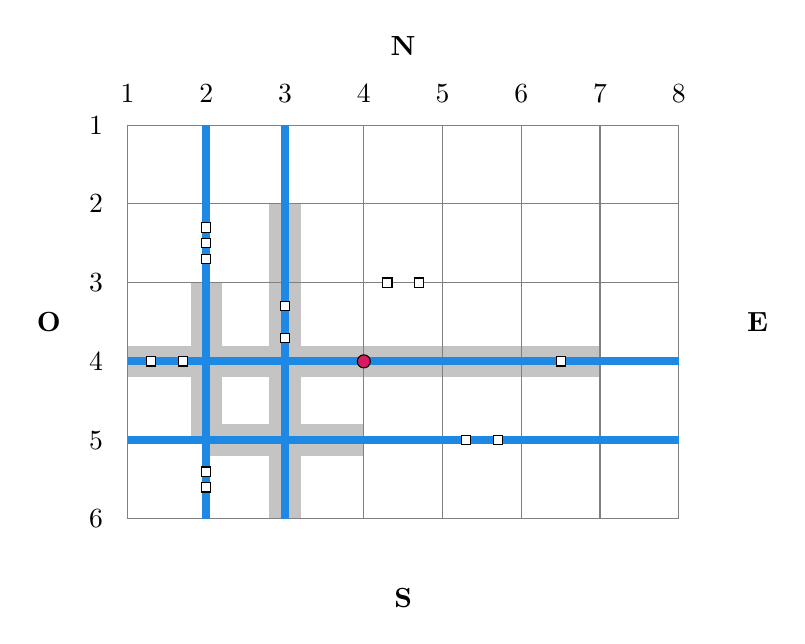
\begin{tikzpicture}
      % Reachable area
      \draw[fill=lightgray, draw opacity=0] (0,1.8) rectangle ++(6, 0.4);
      \draw[fill=lightgray, draw opacity=0] (1,0.8) rectangle ++(2, 0.4);

      \draw[fill=lightgray, draw opacity=0] (1.8,0) rectangle ++(0.4, 4);
      \draw[fill=lightgray, draw opacity=0] (0.8,1) rectangle ++(0.4, 2);

      \def\M{5}
      \def\N{7}
      \draw[gray] (0, 0) grid (\N,\M);
      \foreach \x [count=\i from 1] in {0, ..., \N} {
        \node at (\x, \M + 0.4) {\i};
      }
      \foreach \y [count=\i from 1] in {0, ..., \M} {
        \node at (-0.4, \M - \y) {\i};
      }

      % Sidewalks
      \draw[line width=1mm, draw=blue] (1, 0) to (1, 5);
      \draw[line width=1mm, draw=blue] (2, 0) to (2, 5);
      \draw[line width=1mm, draw=blue] (0, 2) to (7, 2);
      \draw[line width=1mm, draw=blue] (0, 1) to (7, 1);

      % Initial intersection
      \node[circle, draw, fill=red, scale=0.5] at (3, 2) {};

      % Points of interest
      \node[rectangle, draw, fill=white, scale=0.5] at (1, 3.7) {};
      \node[rectangle, draw, fill=white, scale=0.5] at (1, 3.5) {};
      \node[rectangle, draw, fill=white, scale=0.5] at (1, 3.3) {};
      \node[rectangle, draw, fill=white, scale=0.5] at (1, 0.6) {};
      \node[rectangle, draw, fill=white, scale=0.5] at (1, 0.4) {};
      \node[rectangle, draw, fill=white, scale=0.5] at (2, 2.7) {};
      \node[rectangle, draw, fill=white, scale=0.5] at (2, 2.3) {};
      \node[rectangle, draw, fill=white, scale=0.5] at (5.5, 2) {};
      \node[rectangle, draw, fill=white, scale=0.5] at (4.3, 1) {};
      \node[rectangle, draw, fill=white, scale=0.5] at (4.7, 1) {};
      \node[rectangle, draw, fill=white, scale=0.5] at (3.3, 3) {};
      \node[rectangle, draw, fill=white, scale=0.5] at (3.7, 3) {};
      \node[rectangle, draw, fill=white, scale=0.5] at (0.3, 2) {};
      \node[rectangle, draw, fill=white, scale=0.5] at (0.7, 2) {};

      \node at (\N/2, \M + 1) {\bf N};
      \node at (\N/2, -1)     {\bf S};
      \node at (-1, \M/2)     {\bf O};
      \node at (\N + 1, \M/2) {\bf E};
      % \foreach \x [count=\i from 1] in {0, ..., \N} {
      %   \foreach \y [count=\i from 1] in {0, ..., \M} {
      %     \node[circle, draw, fill=white, scale=0.5] at (\x, \y) {};
      %   }
      % }
    \end{tikzpicture}
  }
  \end{center}

  Dadas las calles que tienen vereda, las cuadras en las que están ubicados los puntos de interés
  y la intersección inicial, tu tarea es calcular el nivel de
  acceso para la intersección inicial.
\end{problemDescription}

\begin{inputDescription}
  La primera línea de la entrada contiene dos enteros $M$ y $N$ ($0 < M \leq 100$ y $0 < N\leq 100$)
  correspondientes respectivamente a la cantidad de calles en dirección horizontal y la cantidad de
  calles en dirección vertical.
  La segunda línea contiene $M$ enteros describiendo si las calles en dirección horizontal
  contienen o no una vereda.
  El entero $i$-ésimo será un 1 si la calle $i$ tiene vereda o un 0 en caso contrario.
  Similarmente, la tercera línea contiene $N$ enteros describiendo si las calles en dirección
  vertical contienen veredas.

  La siguiente línea contiene 3 enteros $U$, $V$ y $F$ ($1 \leq U \leq M$, $1 \leq V \leq N$ y $1\leq F \leq 500$).
  El par $(U, V)$ describe la intersección inicial.
  El entero $F$ describe la cantidad máxima de cuadras.
  La intersección $(U, V)$ no necesariamente estará contenida en una calle con vereda.

  A continuación sigue una línea con un entero $E$ ($0 < E \leq 1000$) correspondiente a la cantidad
  de puntos de interés.
  Las siguientes $E$ líneas describen cada una la cuadra en que se encuentra ubicado un punto de interés.
  Cada línea contiene tres enteros $a$, $b$, $c$.
  El par $(a, b)$ representa la intersección de inicio de la cuadra.
  El entero $c$ representa la orientación de la cuadra.
  Si $c$ es 0, la cuadra está en orientada en dirección horizontal, es decir la cuadra está contenida entre las
  intersecciones $(a, b)$ y $(a, b + 1)$.
  Si $c$ es 1, la cuadra está en dirección vertical, es decir, la cuadra está contendida entre
  las intersecciones $(a, b)$ y $(a + 1, b)$.
  Se garantiza que la cuadra siempre estará contenida en la grilla.
\end{inputDescription}

\begin{outputDescription}
  La salida debe contener un único entero mayor o igual que cero indicando el nivel de acceso para
  la intersección inicial, es decir, la cantidad de puntos de interés a una distancia menor o igual
  que $F$ cuadras.
\end{outputDescription}

\begin{scoreDescription}
  \subtask{30}
  Se probarán varios casos donde todas las calles tienen vereda, es decir, la segunda y tercera
  línea de la entrada contendrán solo unos.
  \subtask{70}
  Se probarán varios casos sin restricciones adicionales.
\end{scoreDescription}

\begin{sampleDescription}
\sampleIO{sample-1}
% \sampleIO{sample-2}
\end{sampleDescription}

\end{document}
